\section{Resultados}

En esta sección se muestran los tiempos medidos y los speedup calculados. Los valores que se reportan son la \textbf{mediana} de las 10 corridas, porque es la medida más robusta frente a valores atípicos. Todos los tiempos están en segundos.

\subsection{Tiempos medidos con pthreads}

La tabla~\ref{tab:tiempos-pthreads} muestra el tiempo de la multiplicación para la versión pthreads en segundos.

\begin{table}[ht]
\centering
\begin{tabular}{|c|r|r|r|r|r|}
\hline
\textbf{N} & \textbf{T=1} & \textbf{T=2} & \textbf{T=4} & \textbf{T=8} & \textbf{T=16} \\
\hline
500  & 0.044  & 0.101  & 0.053  & 0.034  & 0.032 \\
1000 & 0.423  & 0.753  & 0.398  & 0.266  & 0.204 \\
2000 & 4.36   & 7.12   & 3.76   & 2.39   & 1.64 \\
4000 & 75.65  & 68.22  & 40.30  & 29.68  & 24.29 \\
8000 & 2441.6 & 690.9  & 416.9  & 354.1  & 401.5 \\
\hline
\end{tabular}
\caption{Tiempos de ejecución con pthreads (segundos, mediana de 10 corridas).}
\label{tab:tiempos-pthreads}
\end{table}

\subsection{Tiempos medidos con fork}

La tabla~\ref{tab:tiempos-fork} muestra lo mismo para la versión fork. No se midió \texttt{T=1} porque es esencialmente la versión secuencial ya medida arriba.

\begin{table}[ht]
\centering
\begin{tabular}{|c|r|r|r|r|}
\hline
\textbf{N} & \textbf{T=2} & \textbf{T=4} & \textbf{T=8} & \textbf{T=16} \\
\hline
500  & 0.029  & 0.022  & 0.015  & 0.015 \\
1000 & 0.239  & 0.143  & 0.130  & 0.117 \\
2000 & 4.86   & 2.36   & 1.98   & 3.01 \\
4000 & 110.5  & 65.3   & 59.1   & 64.6 \\
8000 & 1197.2 & 742.7  & 796.2  & 940.1 \\
\hline
\end{tabular}
\caption{Tiempos de ejecución con fork (segundos, mediana de 10 corridas).}
\label{tab:tiempos-fork}
\end{table}

\subsection{Speedup con pthreads}

La tabla~\ref{tab:speedup-pthreads} muestra el \textit{speedup} de pthreads calculado como tiempo secuencial / tiempo paralelo.

\begin{table}[ht]
\centering
\begin{tabular}{|c|r|r|r|r|}
\hline
\textbf{N} & \textbf{T=2} & \textbf{T=4} & \textbf{T=8} & \textbf{T=16} \\
\hline
500  & 0.44 & 0.83 & 1.27 & 1.40 \\
1000 & 0.56 & 1.06 & 1.59 & 2.07 \\
2000 & 0.61 & 1.16 & 1.83 & 2.66 \\
4000 & 1.11 & 1.88 & 2.55 & 3.11 \\
8000 & 3.53 & 5.86 & 6.90 & 6.08 \\
\hline
\end{tabular}
\caption{Speedup de pthreads.}
\label{tab:speedup-pthreads}
\end{table}

\subsection{Speedup con fork}

La tabla~\ref{tab:speedup-fork} muestra el \textit{speedup} de fork. La base secuencial usada es la misma que para pthreads (\texttt{T=1} de la versión secuencial).

\begin{table}[ht]
\centering
\begin{tabular}{|c|r|r|r|r|}
\hline
\textbf{N} & \textbf{T=2} & \textbf{T=4} & \textbf{T=8} & \textbf{T=16} \\
\hline
500  & 1.54 & 1.99 & 2.89 & 2.88 \\
1000 & 1.77 & 2.95 & 3.25 & 3.62 \\
2000 & 0.90 & 1.85 & 2.20 & 1.45 \\
4000 & 0.69 & 1.16 & 1.28 & 1.17 \\
8000 & 2.04 & 3.29 & 3.07 & 2.60 \\
\hline
\end{tabular}
\caption{Speedup de fork (comparado con el T=1 de pthreads).}
\label{tab:speedup-fork}
\end{table}

\subsection{Comparativa pthreads vs fork}

La tabla~\ref{tab:comparativa} compara directamente las dos técnicas. La columna ``Mejor'' indica qué técnica dio mayor speedup en esa combinación.

\begin{table}[ht]
\centering
\small
\begin{tabular}{|c|c|c|c|c|}
\hline
\textbf{N} & \textbf{T} & \textbf{pthreads} & \textbf{fork} & \textbf{Mejor} \\
\hline
500  & 2  & 0.44 & 1.54 & fork \\
500  & 4  & 0.83 & 1.99 & fork \\
500  & 8  & 1.27 & 2.89 & fork \\
500  & 16 & 1.40 & 2.88 & fork \\
\hline
1000 & 2  & 0.56 & 1.77 & fork \\
1000 & 4  & 1.06 & 2.95 & fork \\
1000 & 8  & 1.59 & 3.25 & fork \\
1000 & 16 & 2.07 & 3.62 & fork \\
\hline
2000 & 2  & 0.61 & 0.90 & fork \\
2000 & 4  & 1.16 & 1.85 & fork \\
2000 & 8  & 1.83 & 2.20 & fork \\
2000 & 16 & 2.66 & 1.45 & pthreads \\
\hline
4000 & 2  & 1.11 & 0.69 & pthreads \\
4000 & 4  & 1.88 & 1.16 & pthreads \\
4000 & 8  & 2.55 & 1.28 & pthreads \\
4000 & 16 & 3.11 & 1.17 & pthreads \\
\hline
8000 & 2  & 3.53 & 2.04 & pthreads \\
8000 & 4  & 5.86 & 3.29 & pthreads \\
8000 & 8  & 6.90 & 3.07 & pthreads \\
8000 & 16 & 6.08 & 2.60 & pthreads \\
\hline
\end{tabular}
\caption{Comparativa de speedup: pthreads vs fork.}
\label{tab:comparativa}
\end{table}

\subsection{Gráficas}

La figura~\ref{fig:speedup-pt} muestra el speedup de la versión pthreads en función del tamaño de la matriz. Se observa que el speedup crece con $N$ y satura cerca de $N = 4000$.

\begin{figure}[ht]
    \centering
    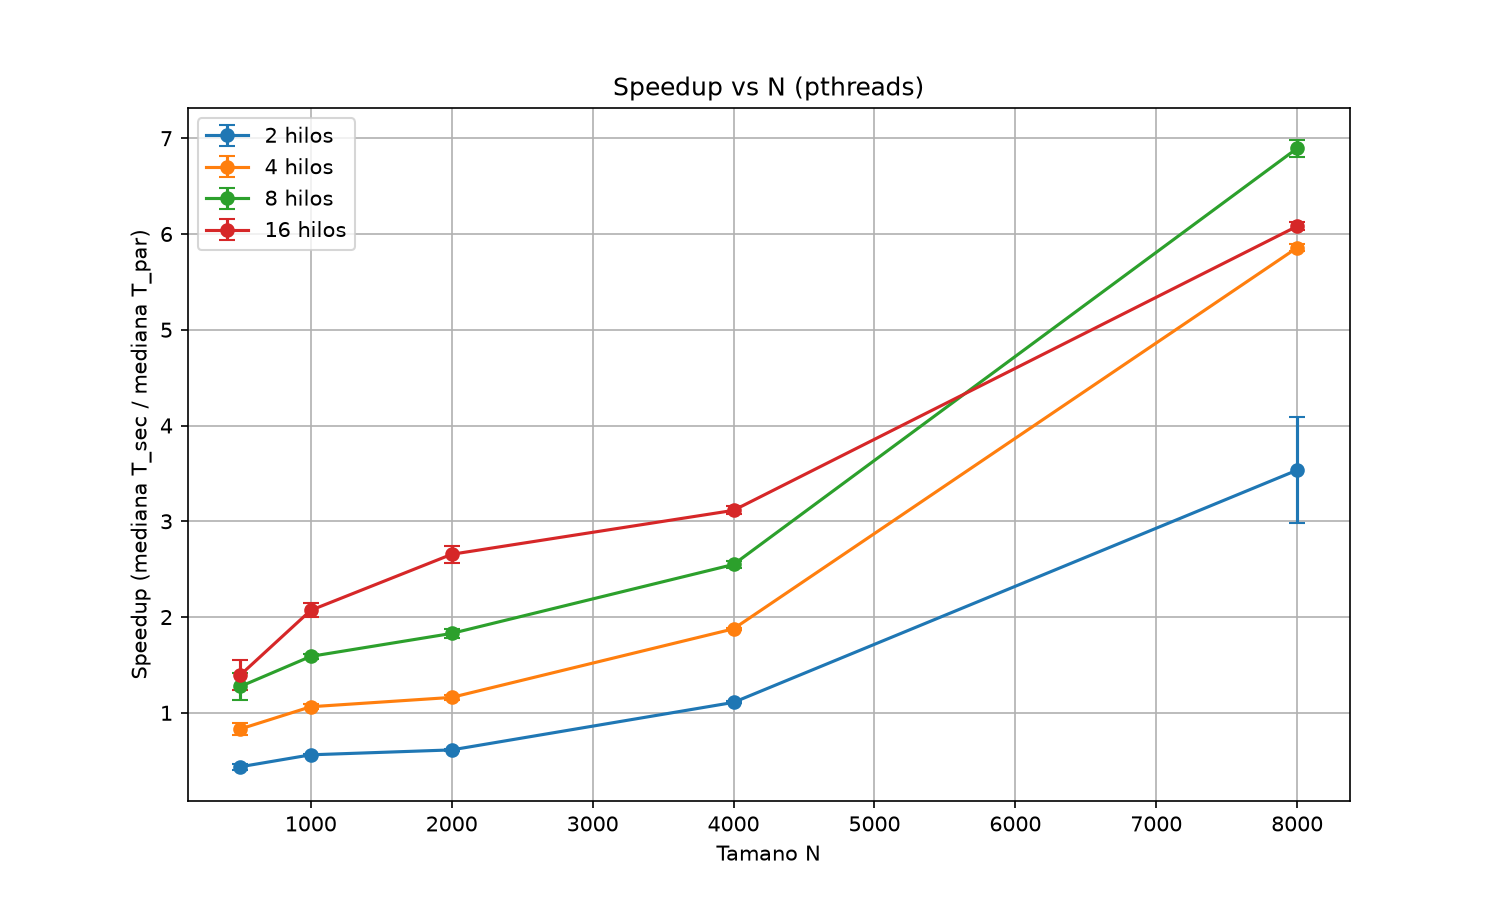
\includegraphics[width=0.85\textwidth]{figuras/speedup_vs_N.png}
    \caption{Speedup de pthreads en función del tamaño de la matriz. Cada curva representa una cantidad fija de hilos.}
    \label{fig:speedup-pt}
\end{figure}

La figura~\ref{fig:speedup-fork} muestra lo mismo para la versión fork. La forma es similar, pero los valores son diferentes: en $N$ chicos el speedup es más alto.

\begin{figure}[ht]
    \centering
    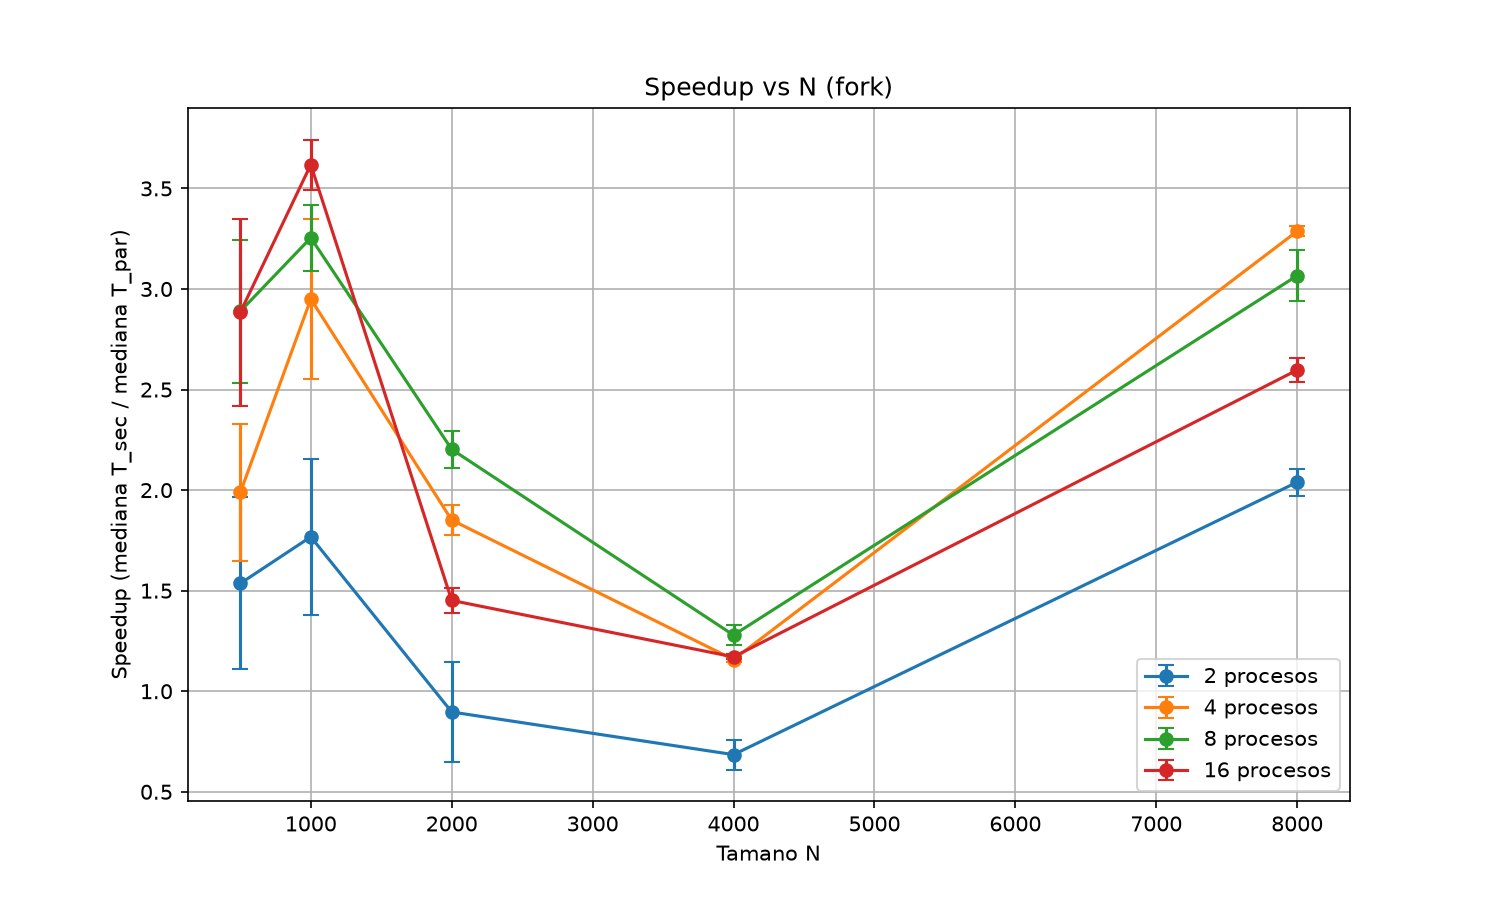
\includegraphics[width=0.85\textwidth]{figuras/speedup_vs_N_fork.png}
    \caption{Speedup de fork en función del tamaño de la matriz.}
    \label{fig:speedup-fork}
\end{figure}

La figura~\ref{fig:comparativa-plot} es la gráfica principal de este trabajo: muestra las 8 curvas (4 de pthreads y 4 de fork) en una sola imagen para facilitar la comparación directa.

\begin{figure}[ht]
    \centering
    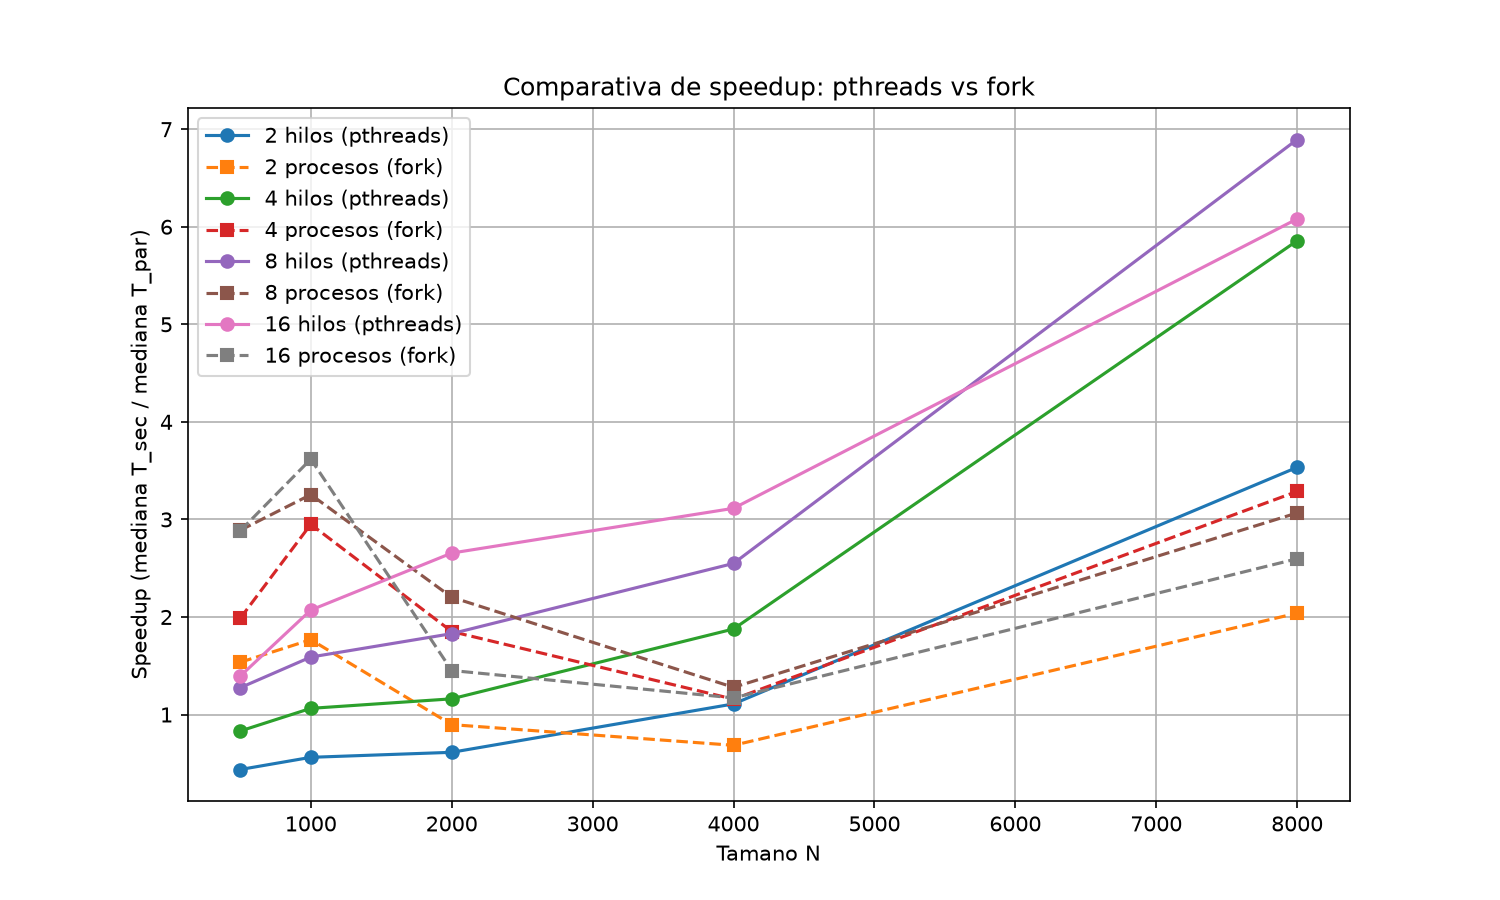
\includegraphics[width=0.85\textwidth]{figuras/speedup_comparativa.png}
    \caption{Comparativa de speedup: pthreads vs fork. Las líneas continuas con círculos son pthreads, las líneas punteadas con cuadrados son fork.}
    \label{fig:comparativa-plot}
\end{figure}

\subsection{Outliers detectados}

Al revisar las 10 corridas individuales de cada configuración con fork, se identificaron cinco valores atípicos puntuales. Todos corresponden a la \textbf{corrida número 10} de las configuraciones con $T = 2$. La tabla~\ref{tab:outliers} los resume.

\begin{table}[ht]
\centering
\begin{tabular}{|l|c|c|c|}
\hline
\textbf{Configuración} & \textbf{Outlier} & \textbf{Tiempo típico} & \textbf{Desviación} \\
\hline
N=500, T=2, run=10   & 0.057 s & $\sim$0.029 s & casi 2$\times$ \\
N=1000, T=2, run=10  & 0.426 s & $\sim$0.244 s & 80\% arriba \\
N=2000, T=2, run=10  & 9.84 s  & $\sim$4.86 s  & \textbf{el doble} \\
N=4000, T=2, run=10  & 152 s   & $\sim$110 s   & 37\% arriba \\
N=8000, T=2, run=10  & 1327 s  & $\sim$1197 s  & 11\% arriba \\
\hline
\end{tabular}
\caption{Valores atípicos puntuales en fork, todos en T=2 run=10.}
\label{tab:outliers}
\end{table}

Que todos los outliers caigan en la corrida 10 de las configuraciones con $T = 2$ sugiere que se debió a \textbf{ruido del sistema} en una ventana de tiempo específica (otra tarea puntual del sistema operativo), no a un problema del programa. El uso de la \textbf{mediana} como medida central hace que estos picos no distorsionen el speedup reportado, mientras que la media se vería fuertemente afectada.
